%%%%%%%%%%%%%%%%%%%%%%%%%%%%%%%%%%%%%%%%%
% Beamer Presentation
% LaTeX Template
% Version 1.0 (10/11/12)
%
% This template has been downloaded from:
% http://www.LaTeXTemplates.com
%
% License:
% CC BY-NC-SA 3.0 (http://creativecommons.org/licenses/by-nc-sa/3.0/)
%
%%%%%%%%%%%%%%%%%%%%%%%%%%%%%%%%%%%%%%%%%

%----------------------------------------------------------------------------------------
%	PACKAGES AND THEMES
%----------------------------------------------------------------------------------------

\documentclass{beamer}

\mode<presentation> {

% The Beamer class comes with a number of default slide themes
% which change the colors and layouts of slides. Below this is a list
% of all the themes, uncomment each in turn to see what they look like.

%\usetheme{default}
%\usetheme{AnnArbor}
%\usetheme{Antibes}
%\usetheme{Bergen}
%\usetheme{Berkeley}
%\usetheme{Berlin}
%\usetheme{Boadilla}
%\usetheme{CambridgeUS}
%\usetheme{Copenhagen}
%\usetheme{Darmstadt}
%\usetheme{Dresden}
%\usetheme{Frankfurt}
%\usetheme{Goettingen}
%\usetheme{Hannover}
%\usetheme{Ilmenau}
%\usetheme{JuanLesPins}
%\usetheme{Luebeck}
\usetheme{Madrid}

\usepackage{listings} % Required for insertion of code
%\usetheme{Malmoe}
%\usetheme{Marburg}
%\usetheme{Montpellier}
%\usetheme{PaloAlto}
%\usetheme{Pittsburgh}
%\usetheme{Rochester}
%\usetheme{Singapore}
%\usetheme{Szeged}
%\usetheme{Warsaw}

% As well as themes, the Beamer class has a number of color themes
% for any slide theme. Uncomment each of these in turn to see how it
% changes the colors of your current slide theme.

%\usecolortheme{albatross}
%\usecolortheme{beaver}
%\usecolortheme{beetle}
%\usecolortheme{crane}
%\usecolortheme{dolphin}
%\usecolortheme{dove}
%\usecolortheme{fly}
%\usecolortheme{lily}
%\usecolortheme{orchid}
%\usecolortheme{rose}
%\usecolortheme{seagull}
%\usecolortheme{seahorse}
%\usecolortheme{whale}
%\usecolortheme{wolverine}

%\setbeamertemplate{footline} % To remove the footer line in all slides uncomment this line
%\setbeamertemplate{footline}[page number] % To replace the footer line in all slides with a simple slide count uncomment this line

%\setbeamertemplate{navigation symbols}{} % To remove the navigation symbols from the bottom of all slides uncomment this line
}

\usepackage{graphicx} % Allows including images
\usepackage{booktabs} % Allows the use of \toprule, \midrule and \bottomrule in tables

%----------------------------------------------------------------------------------------
%	TITLE PAGE
%----------------------------------------------------------------------------------------

\title[Introduzione]{Design Pattern} % The short title appears at the bottom of every slide, the full title is only on the title page

\author{Claudio Menghi,  Srdan Krstic} % Your name
\institute[Deepse group] % Your institution as it will appear on the bottom of every slide, may be shorthand to save space
{
Politecnico di Milano \\ % Your institution for the title page
\medskip
\textit{menghi@elet.polimi.it,  srdan.krstic@polimi.it} % Your email address
}
\date{\today} % Date, can be changed to a custom date

\begin{document}

\begin{frame}
\titlepage % Print the title page as the first slide
\end{frame}

\begin{frame}
\frametitle{Overview} % Table of contents slide, comment this block out to remove it
\tableofcontents % Throughout your presentation, if you choose to use \section{} and \subsection{} commands, these will automatically be printed on this slide as an overview of your presentation
\end{frame}

%----------------------------------------------------------------------------------------
%	PRESENTATION SLIDES
%----------------------------------------------------------------------------------------

\section{Introduction}

\begin{frame}
\frametitle{Patterns}
Structural	Patterns\\
\begin{itemize}
\item Adapter:	Match	interfaces	of	different	classes	
\item Bridge:	Separates	an	object’s	interface	from	its	 implementation	
\item Composite:	A	tree	structure	of	simple	and	composite	objects	
\item Decorator:	Add	responsibilities	to	objects	dynamically	
\item  Facade:	A	single	class	 that	 represents	an	 entire	subsystem
\item Flyweight:	A	fine-grained	instance	used	for	efficient	sharing	
\item Proxy:	An	object	representing	 another	object	
\end{itemize}	
\end{frame}

\begin{frame}
\frametitle{Patterns}
Behavioral	Patterns\\
\begin{itemize}
\item Chain	of	Resp.:	A	way	of	passing	a	request	between	a	chain	of	objects
\item Command:	Encapsulate	a	command	request	as	an	object		
\item Interpreter:	A	way	to	include	language	elements	in	a	program	
\item Iterator:	Sequentially	access	the	elements	of	a	collection	
\item Mediator:	Defines	simplified	communication 	between	classes	
\item Memento:	Capture	and	restore	an	object's	internal	state	
\item Observer:	A	way	of	notifying	change	to	a	number	of	classes	
\item State:	Alter	an	object's	behavior	when	its	state	changes
\item Strategy:	Encapsulates	an	algorithm	inside	a	class
\item Template	Method:	Defer	the	exact	steps	of	an	algorithm	to	a	subclass	
\item Visitor:	Defines	a	new	operation	to	a	class	without	change	
\end{itemize}	
\end{frame}

\section{Esercizio 1}

\begin{frame}
\frametitle{Esercizio 1}
Esercizio 1: 
\begin{itemize}
\item Vogliamo sviluppare una applicazione che permetta l'utilizzo di diverse tecnologie di comunicazione, evitando il pi\`u possibile duplicazioni di codice
\item come possiamo strutturare la nostra applicazione?
\item supponiamo per esempio di avere la nostra logica che ci consente di eseguire un set di operazione \texttt{action(A)},  \texttt{action(B)} and  \texttt{action(C)} come possiamo supportare un client che utilizza dei comandi specificati per mezzo di Stringhe o vari tipi di comunicazione?  
\end{itemize}
\end{frame}


\begin{frame}
\frametitle{Esercizio 1}
\begin{figure}
\centering
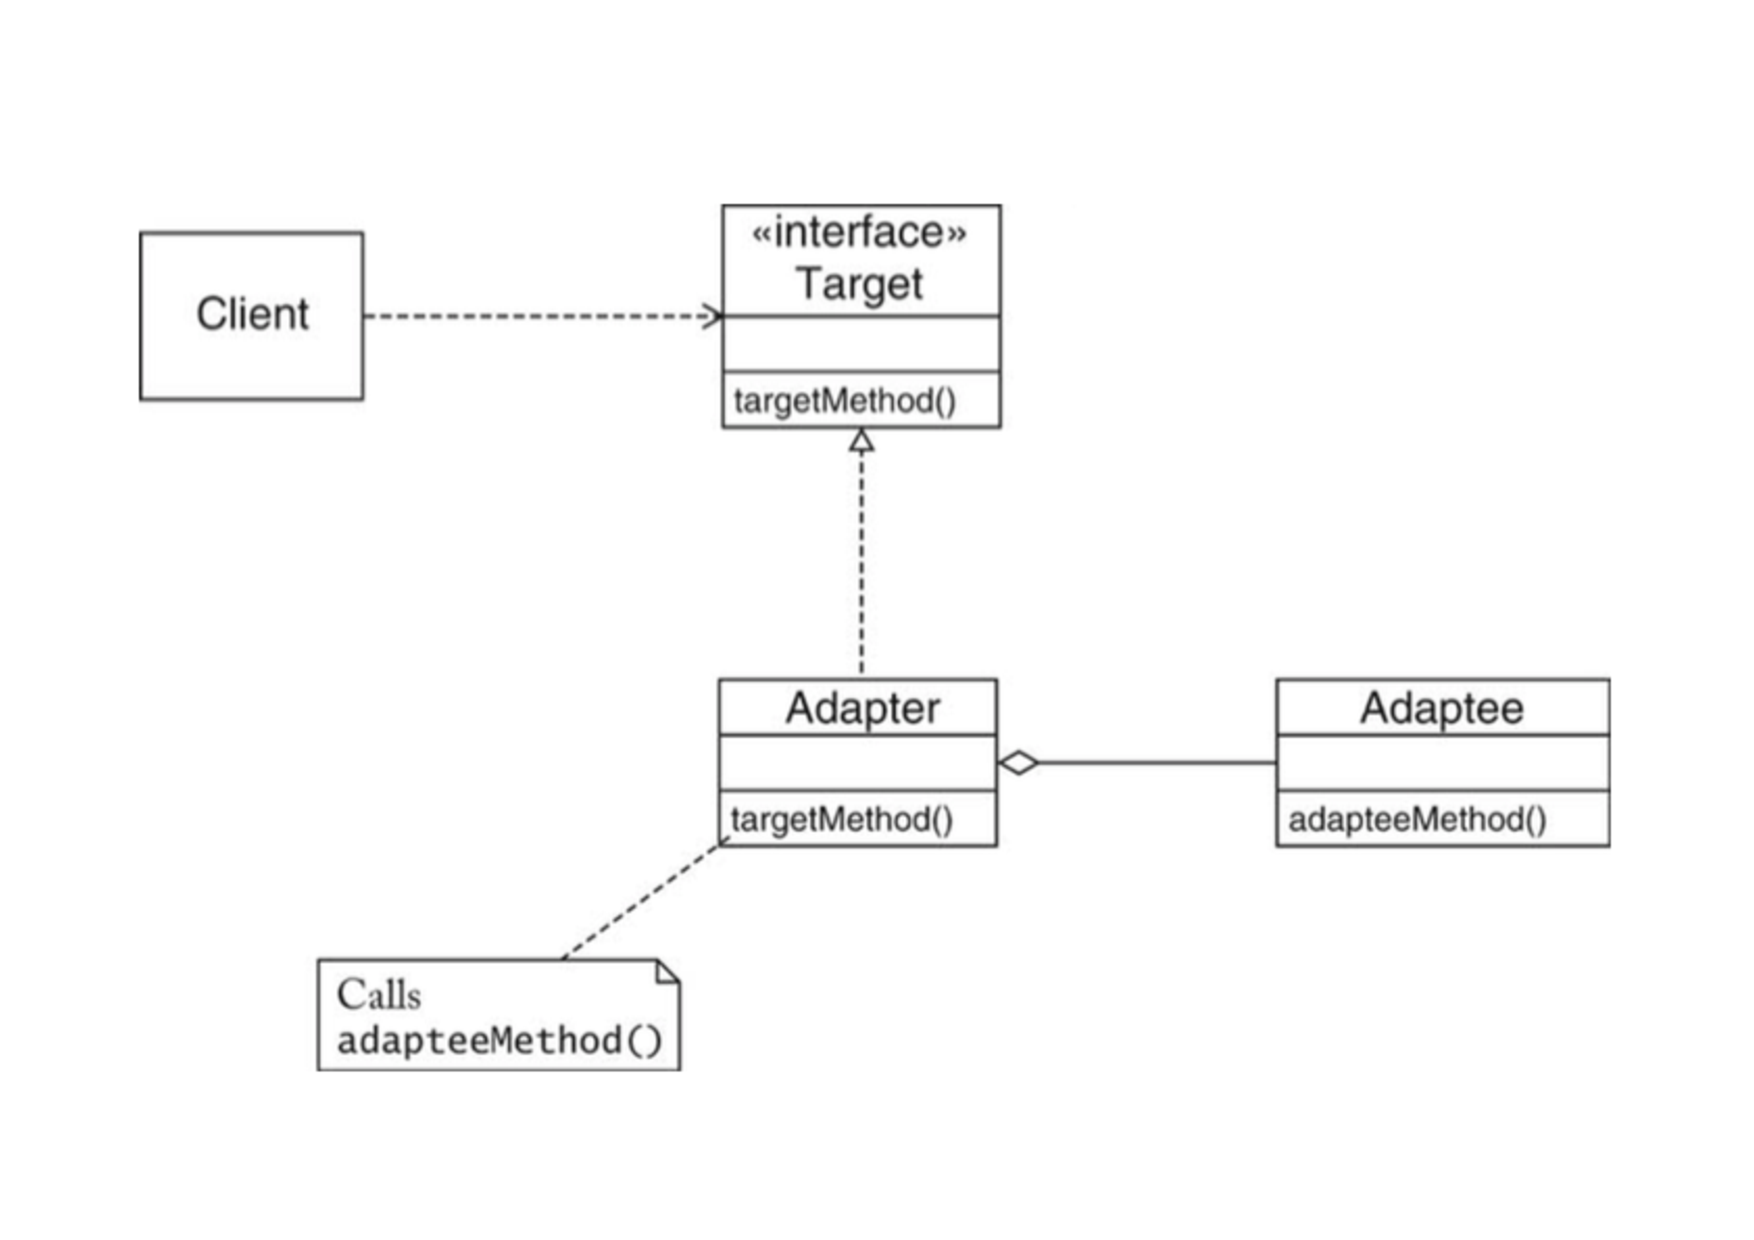
\includegraphics[width=0.7\textwidth]{Img/Adapter.pdf}
\caption{Class diagram relativo al pattern Adapter}
\label{Fig:FactoryAdapterConcepts}
\end{figure}
\end{frame}


\section{Esercizio 2}
\begin{frame}
\frametitle{Esercizio 2}
Esercizio 2: Immaginiamo di implementare un social network. Data una specifica persona vorremmo mostrare come ``potenziali amici" gli  amici degli amici degli amici. Come possiamo implementarla in maniera efficace?
\end{frame}

\begin{frame}
\frametitle{Esercizio 2}
\begin{figure}
\centering
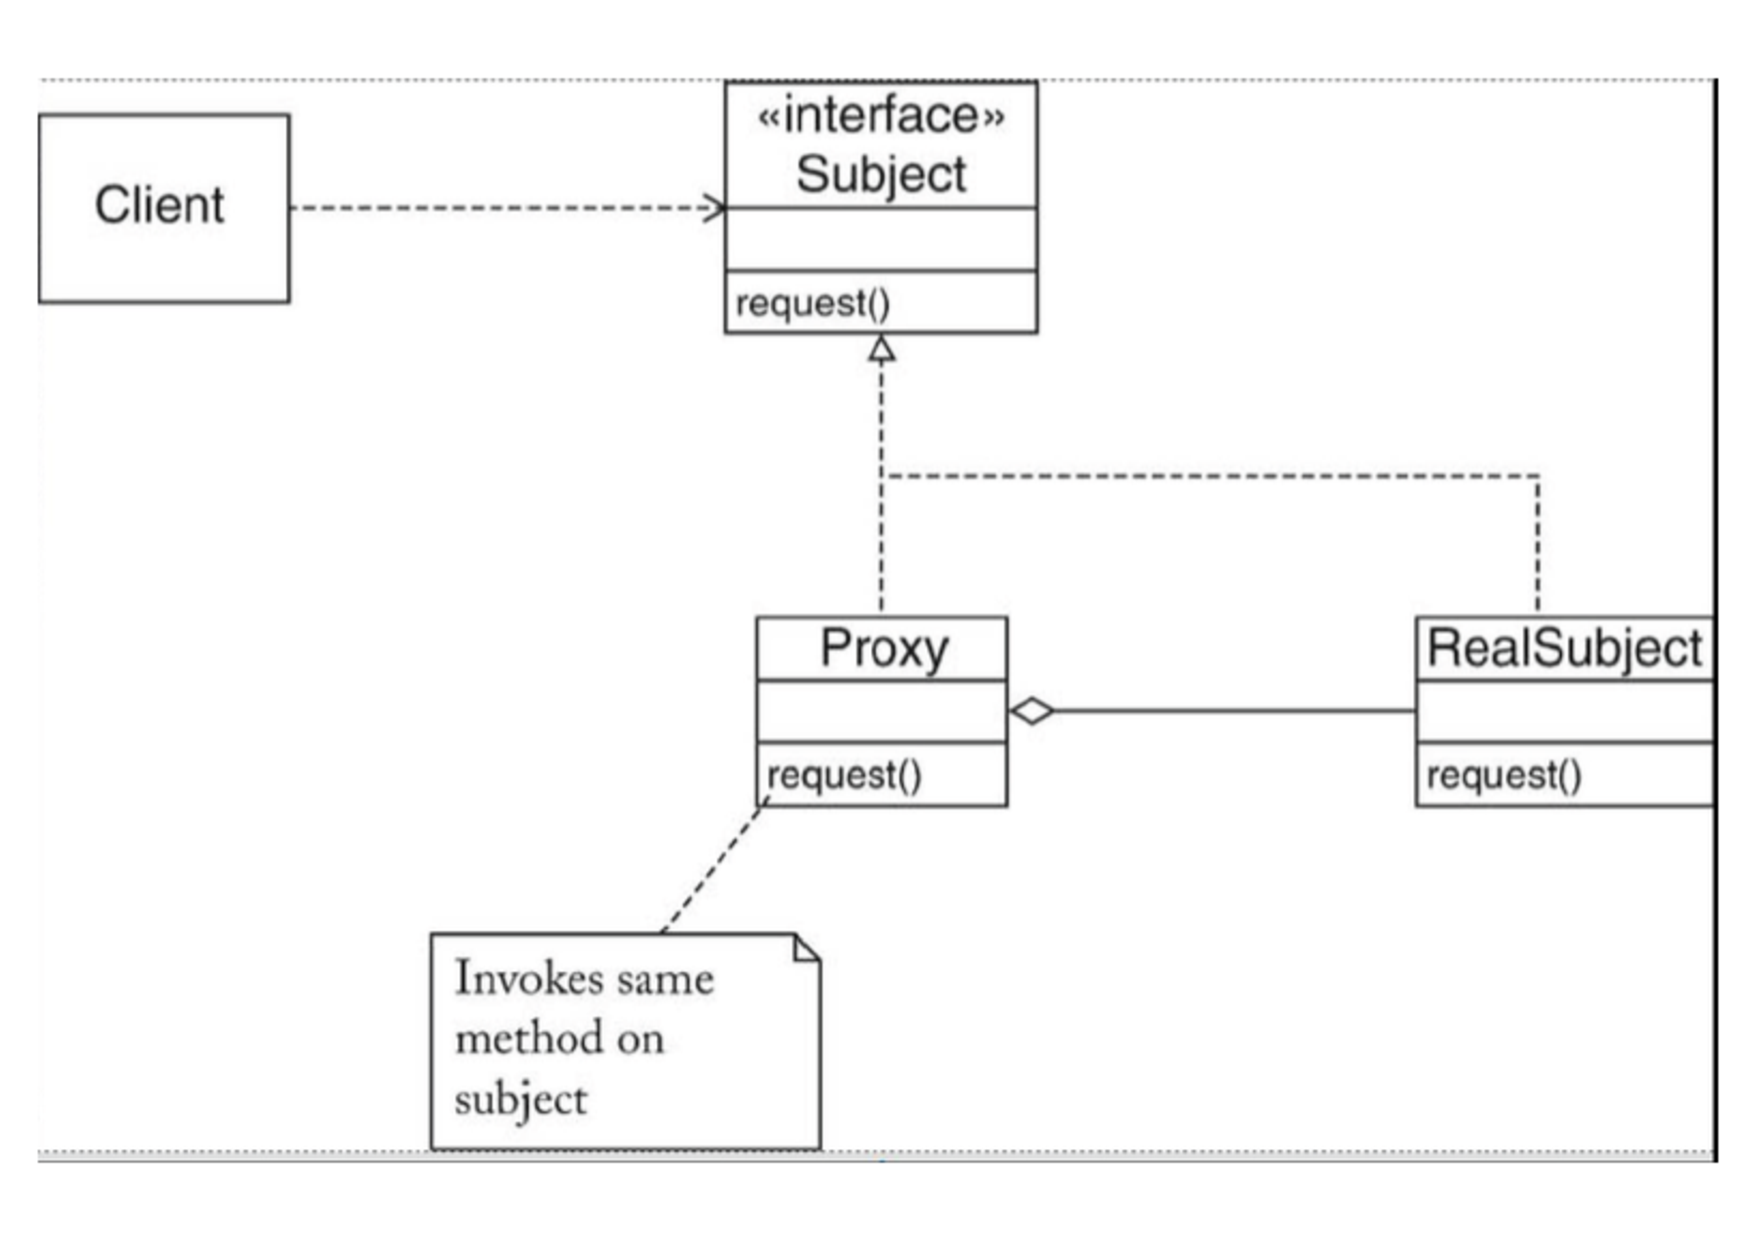
\includegraphics[width=0.7\textwidth]{Img/Proxy.pdf}
\caption{Class diagram relativo al pattern Proxy}
\label{Fig:ProxyAdapterConcepts}
\end{figure}
\end{frame}

\section{Esercizio 3}
\begin{frame}
\frametitle{Esercizio 3}
Esercizio 3: Scrivere un applicazione per rappresentare diversi tipi di caff\`e con diversi ingredienti. Per esempio, vorremmo aggiungere del caramello, del whiskey, dello zucchero, a richiesta.
\end{frame}

\begin{frame}
\frametitle{Esercizio 3}
\begin{figure}[h]
\centering
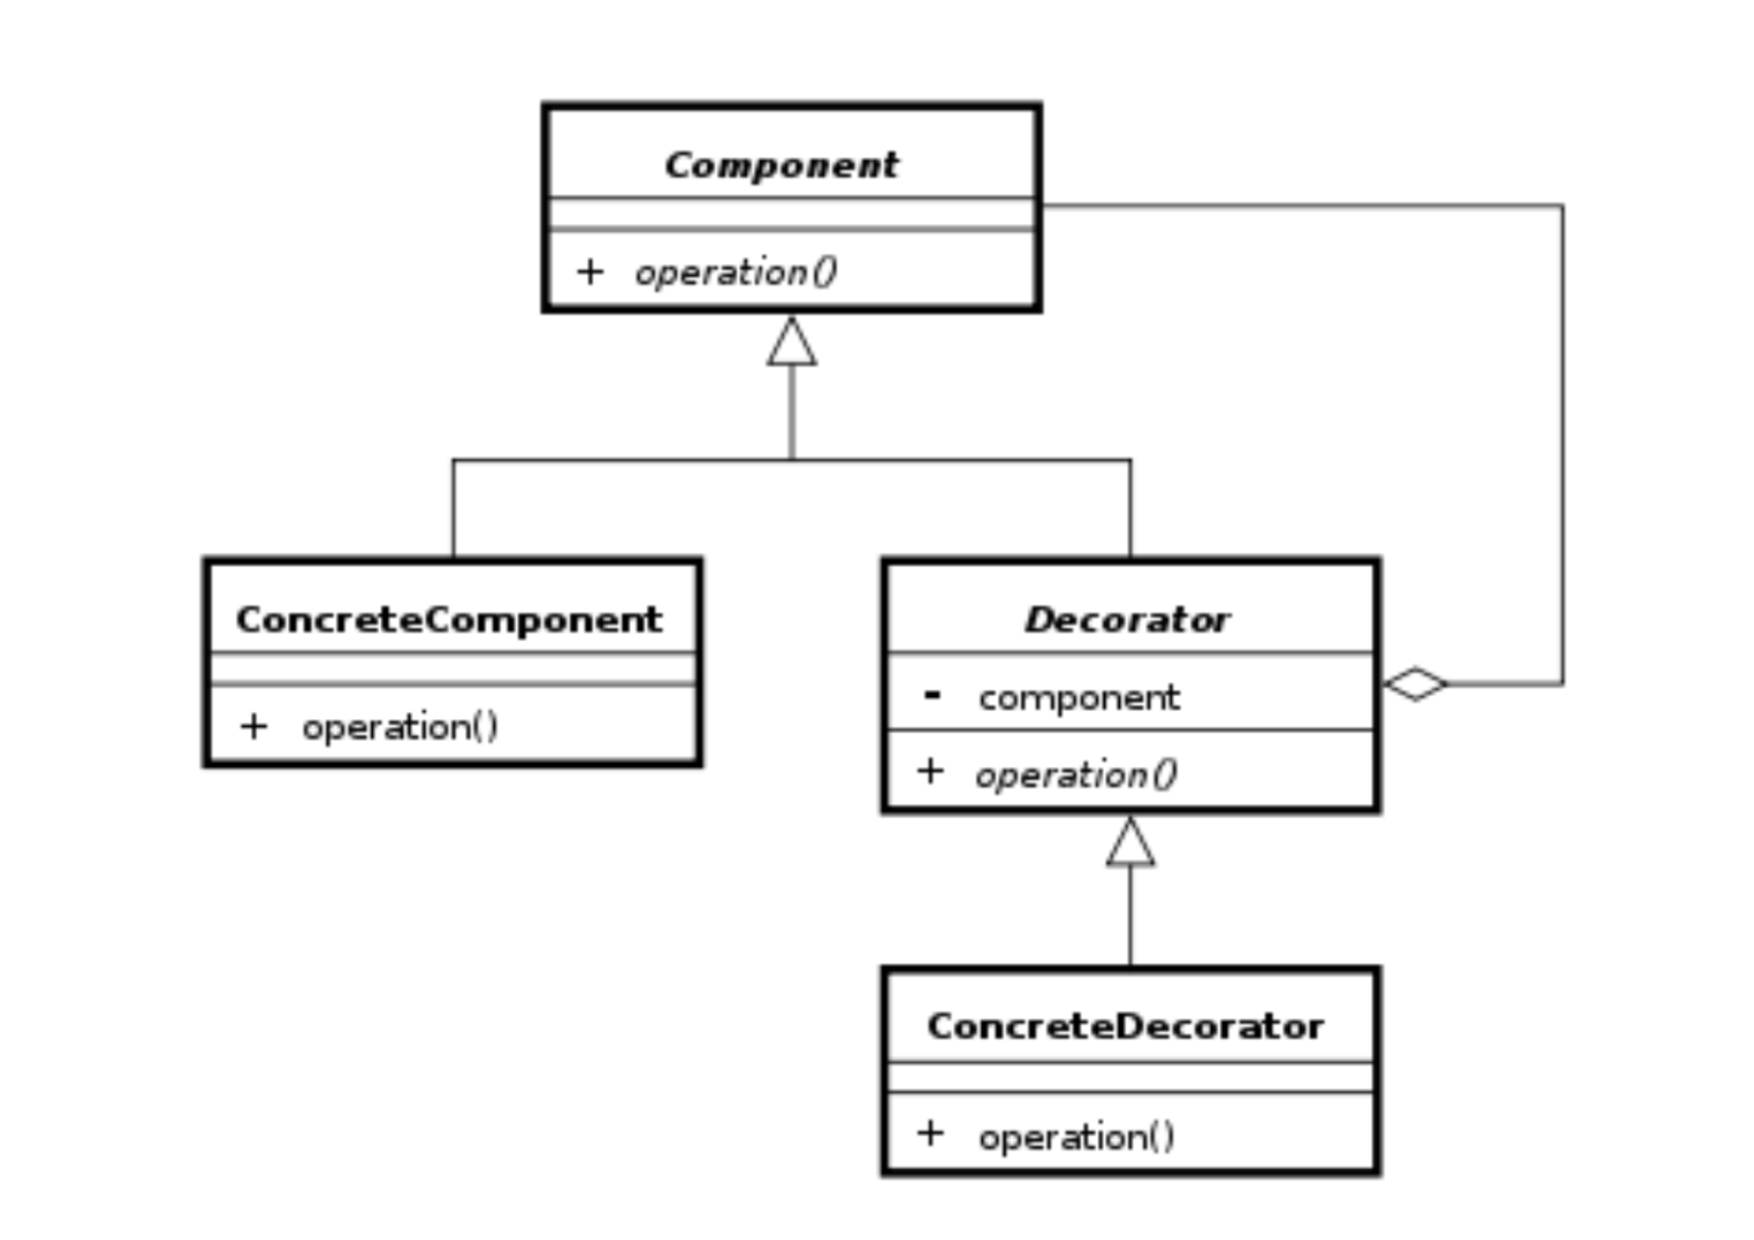
\includegraphics[width=0.7\textwidth]{Img/Decorator.pdf}
\caption{Class diagram relativo al pattern Decorator}
\label{Fig:DecoratorConcepts}
\end{figure}
\end{frame}


\section{Esercizio 4}
\begin{frame}
\frametitle{Esercizio 4}
Esercizio 4: scrivere il codice per rappresentare un robot che pu\`o avere diverse strategie per gestire il suo comportamento. Vogliamo fare si che i comportamenti possano cambiare mentre la nostra applicazione \`e in esecuzione.
\end{frame}

\begin{frame}
\frametitle{Esercizio 4}
\begin{figure}[h]
\centering
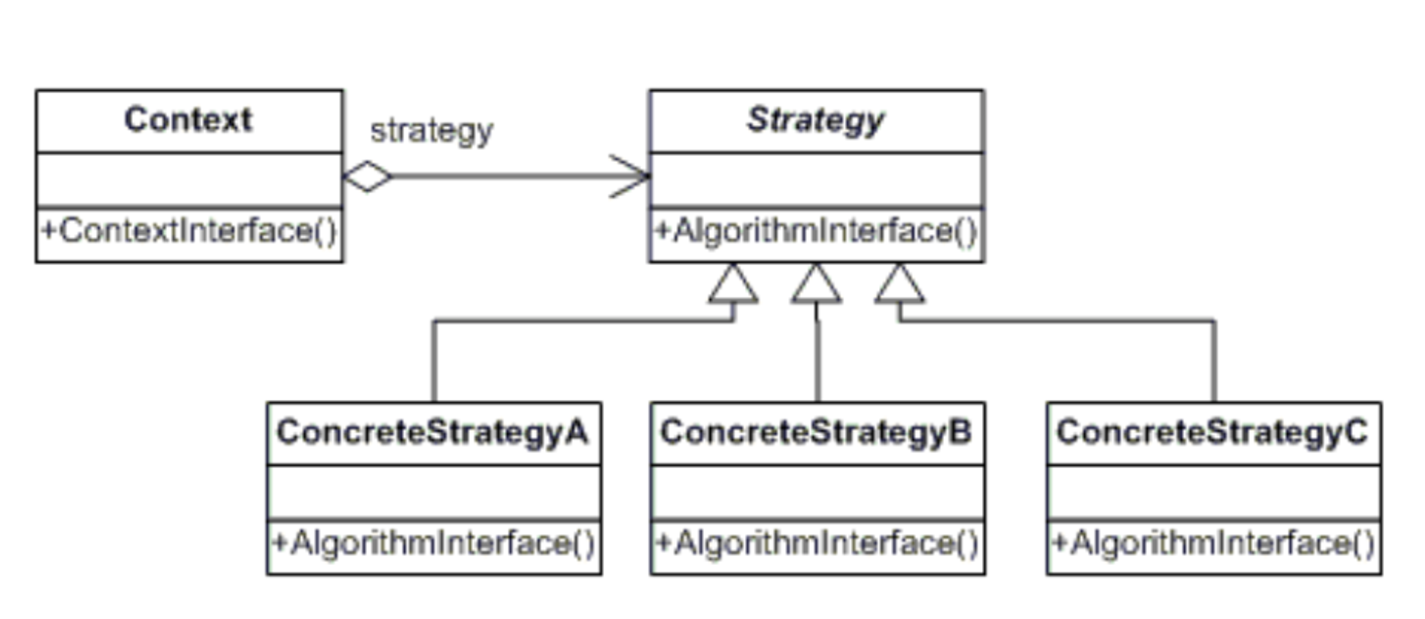
\includegraphics[width=0.7\textwidth]{Img/Strategy.pdf}
\caption{Class diagram relativo al pattern Strategy}
\label{Fig:StrategyConcepts}
\end{figure}
\end{frame}

\section{Esercizio 5}
\begin{frame}
\frametitle{Esercizio 5}
Progettare un sistema per il monitoraggio del Meteo:
\begin{itemize}
\item si ha a disposizione l'oggetto \texttt{WeatherData} che fornisce temperatura, umidit\`a, pressione
\item implementare tre diversi tipi di display che mostrano condizione attuale, previsioni e statistiche
\item il sistema deve essere espandibile per supportare nuovi display
\end{itemize}
\end{frame}

\begin{frame}
\frametitle{Esercizio 5}
\begin{figure}[h]
\centering
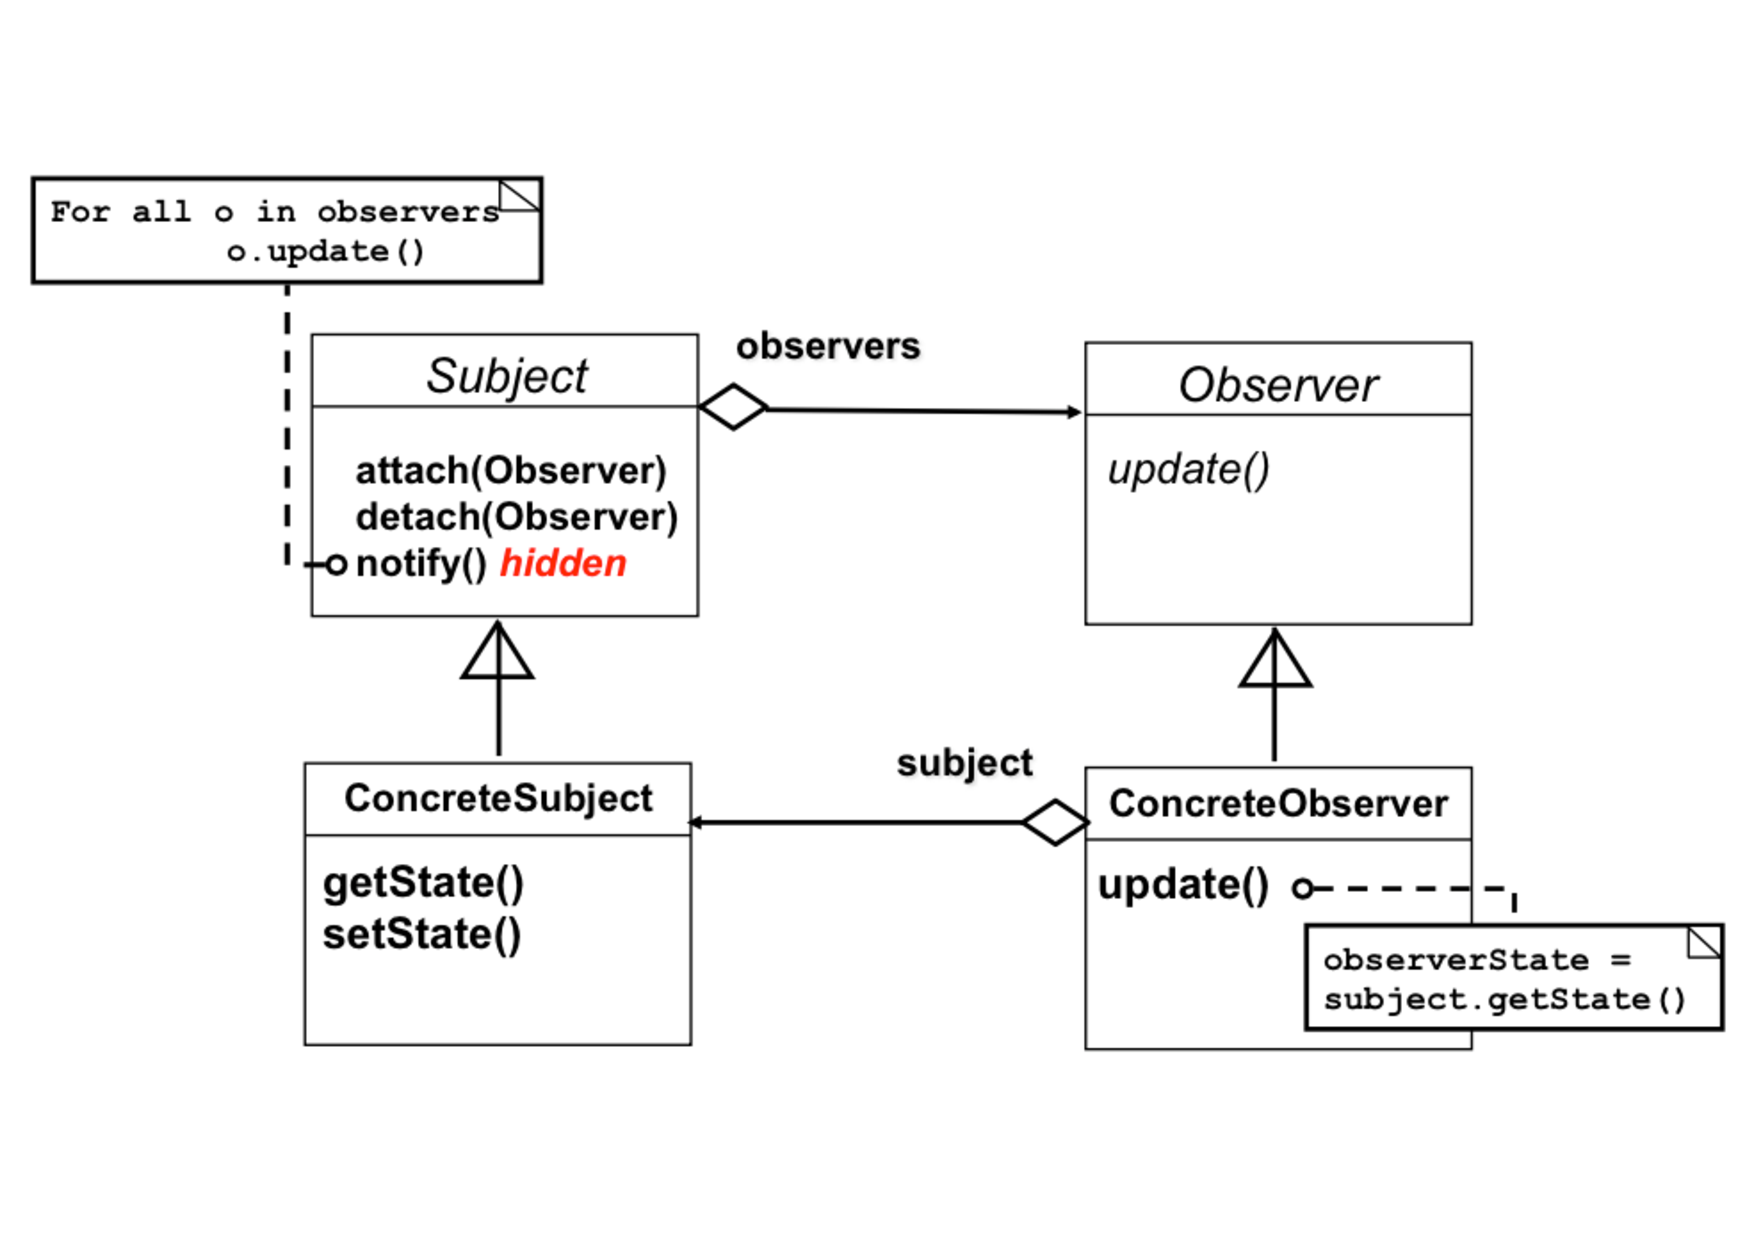
\includegraphics[width=0.7\textwidth]{Img/Observer.pdf}
\caption{Class diagram relativo al pattern Observer}
\label{Fig:ObserverConcepts}
\end{figure}
\end{frame}

\section{Esercizio 6}
\begin{frame}
\frametitle{Esercizio 6}
Supponendo che sia definita la classe:

\emph{public class Matrix {\\
	public int rows(){ /**/ }\\
	public int columns(){  /**/ }\\
	public float element(int row, int column){/**/}\\
}}
Si scriva in Java un opportuno iteratore che gestisca l’accesso sequenziale (per riga) agli elementi della matrice
\begin{figure}[h]
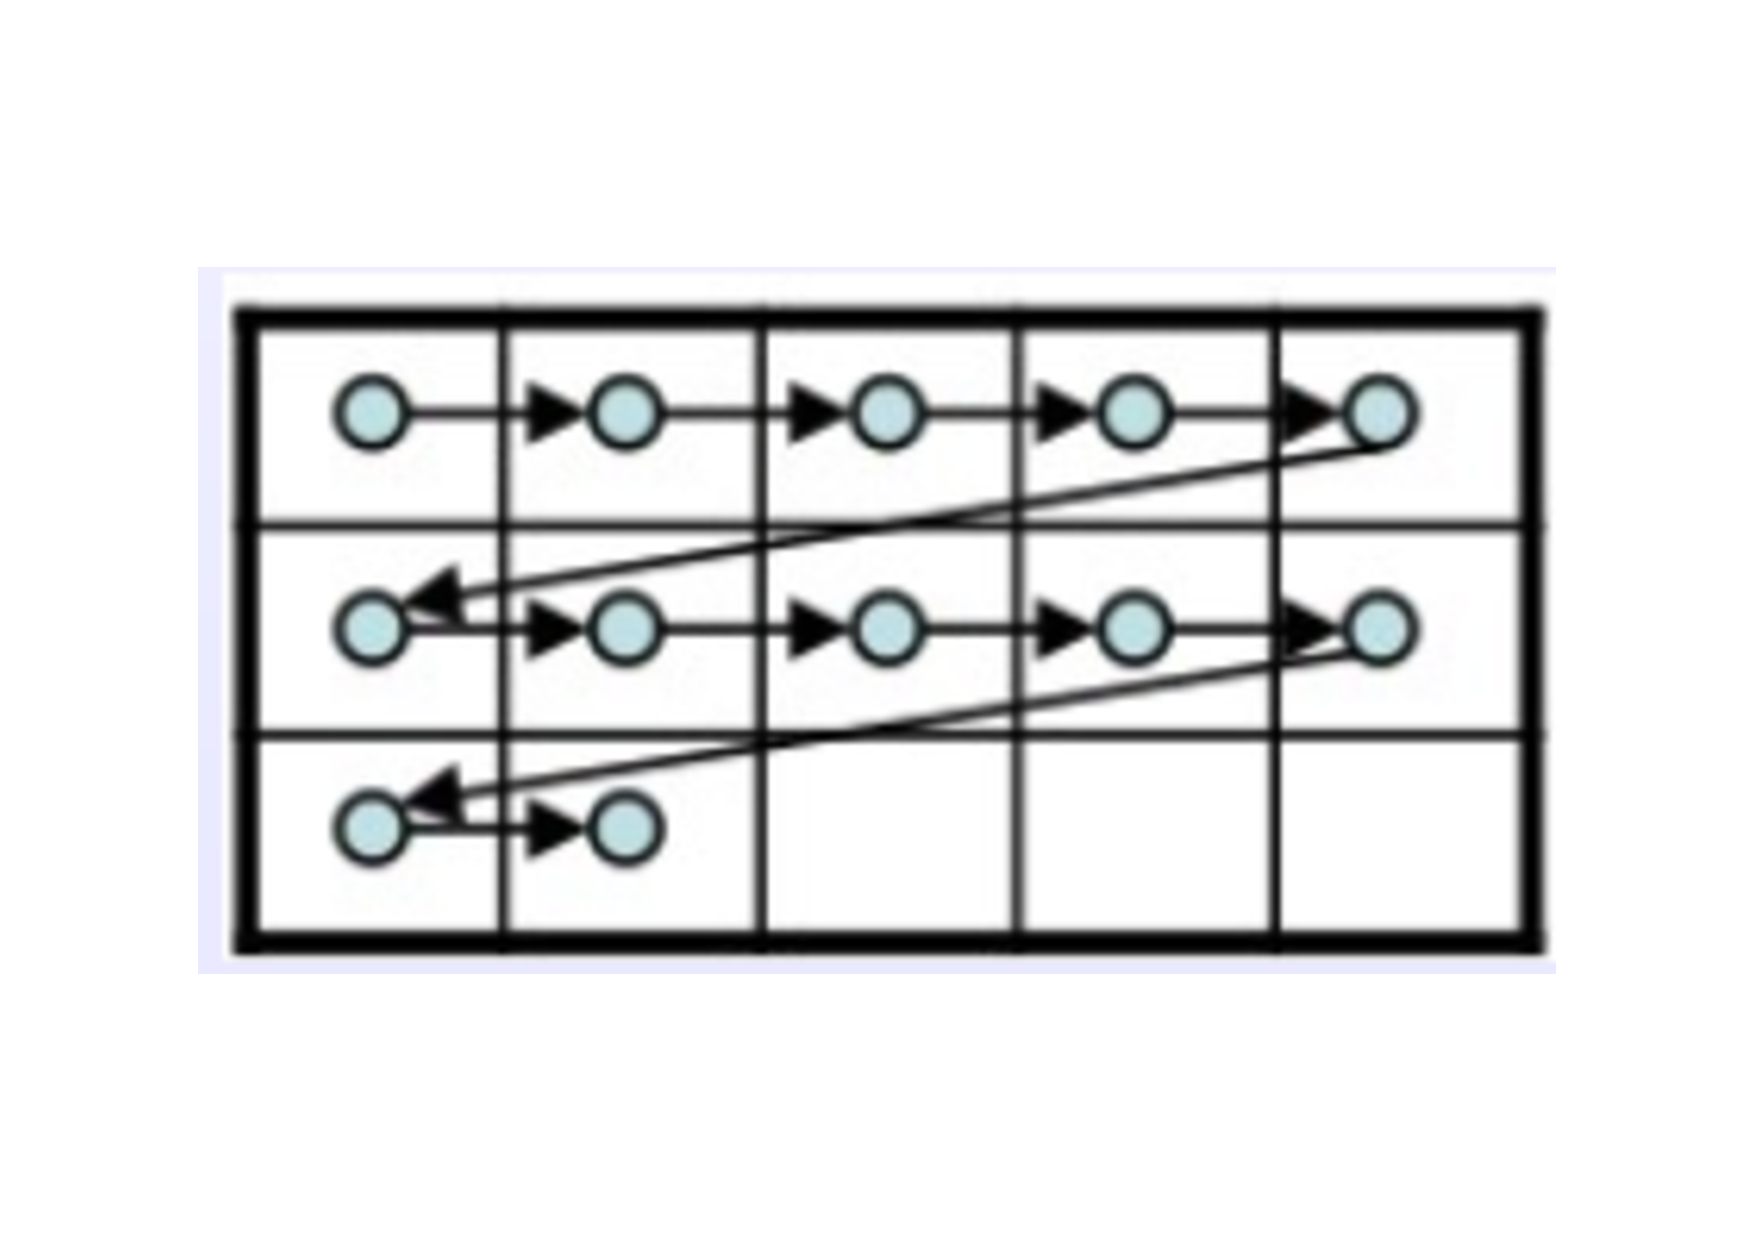
\includegraphics[width=0.4\textwidth]{Img/Matrix.pdf}
\end{figure}
\end{frame}





%----------------------------------------------------------------------------------------

\end{document} 